\documentclass[conference]{IEEEtran}
\usepackage{cite}
\usepackage{graphicx}
\usepackage{booktabs}
\usepackage{url}
\usepackage{tikz}
\usetikzlibrary{arrows.meta,positioning}

\title{Restoring Corrupted Pet Photographs with a Universal Autoencoder, Hard Routing, and a Soft Mixture of Experts}

\author{\IEEEauthorblockN{Ibraheem Farooq}\\
\IEEEauthorblockA{23i-0816}}

\begin{document}
\maketitle

\begin{abstract}
Three restorers were trained on the same Oxford-IIIT Pet split and the same four corruptions, which are clean, salt and pepper, Gaussian blur, and rectangular occlusion. One denoising autoencoder helps on salt and on occlusion, and on blur it is worse than leaving the image alone. A classifier with three specialists, plus a bypass that returns clean images unchanged, is stronger overall, and blur is still not fixed. The soft mixture starts from those specialists. After two warm-up epochs and eight fine-tuning epochs it reaches test L1 0.0291 and SSIM 0.863, which is better than both earlier models on those two scores. PSNR is 28.7, below hard routing at 30.5, because a clean photo is no longer copied through unchanged. The face-to-sketch model and the video demo were not finished.
\end{abstract}

\begin{IEEEkeywords}
denoising autoencoder, mixture of experts, image restoration
\end{IEEEkeywords}

\section{Introduction}
The assignment asks for four models. This paper only covers the three that restore pet photos. Those models have to repair damage, and the first of them is not told which damage was applied. The later models are compared with the earlier ones on one frozen test list, so the comparison is on the same images.

The first model is a convolutional autoencoder. Hard routing adds a four-class classifier and a separate autoencoder for each kind of damage. The soft mixture keeps those specialists, adds a branch that returns the input, and mixes the four outputs with a softmax. Task~4 is the face-to-sketch GAN, and it is not included here.

\section{Related research}
A denoising autoencoder is trained to rebuild a clean image from a damaged one, so the hidden map has to keep what stays stable in the photo and drop the noise~\cite{vincent2008}. SSIM looks at structure instead of only the pixel error, and the restoration losses in this project mix L1 with SSIM for that reason~\cite{wang2004}.

Mixtures of experts send different inputs toward different models~\cite{jacobs1991}. Hard routing picks a single expert. A soft mixture adds the expert outputs with weights, so more than one expert can affect the image. Later networks use sparse gates for the same idea~\cite{shazeer2017}. The gate here is a small classifier. The assignment wants all four weights on every image, so a top-$k$ gate would leave some of them out.

The photos are from Oxford-IIIT Pet~\cite{parkhi2012}. Breed labels are not used. The clean photo is the image the model is trained to match.

\section{Dataset preparation}
The official trainval list and the official test list are kept apart. Trainval is shuffled with seed 42 and then split 80/20, which gives 2{,}944 training images and 736 validation images. The test list has 3{,}669 images. It is not used for training, and it is not used to pick settings. Each image is converted to RGB and resized to $128\times128$ with bicubic interpolation, stretched to a square. The clean copies are saved as PNG so a second JPEG save does not add more damage.

Training corruption is drawn when an image is loaded, with equal chance for each of the four conditions. Validation damage and test damage are written once into manifest files and then left alone. The test manifest has ten rows for every image, in the order shown in Table~\ref{tab:corrupt}.

\begin{table}[t]
\caption{Frozen test corruptions. Occlusion coverage is within one percentage point of the target.}
\label{tab:corrupt}
\centering
\small
\begin{tabular}{@{}lll@{}}
\toprule
Corruption & Severity & Setting \\
\midrule
Clean & none & unchanged \\
Salt & low / med / high & $p=0.03$ / $0.08$ / $0.15$ \\
Blur & low / med / high & $k=3,5,7$; $\sigma=0.7,1.5,2.5$ \\
Occlusion & low / med / high & 1, 2, or 3 boxes \\
\bottomrule
\end{tabular}
\end{table}

Salt turns chosen pixels black or white. One decision is made per pixel and shared by all channels. Blur is a separable Gaussian with reflect padding. Occlusion draws black rectangles that do not overlap. Low, medium, and high occlusion use 1, 2, and 3 rectangles, covering about 10\%, 20\%, and 35\% of the image. Training, the manifest files, and the web app all call the same functions, so the damage rules are not rewritten in three places.

\section{Architecture}
\subsection{Universal autoencoder}
The encoder is a stack of $7\times7$ convolutions with stride 2. The first layer has 256 channels, and the next layer doubles that. The bottleneck is a $32\times32$ map. The decoder mirrors the encoder with transposed convolutions and ends in a sigmoid. There are no skip connections, and the norm is group norm. The map holds about 10.7 times as many values as the $128\times128\times3$ input, so it does not squeeze the image. The brief asks for a real bottleneck, and this one does not meet that, which has to be stated as a limitation.

\subsection{Hard routing}
The classifier is four stride-2 conv blocks with base width 32, then global average pooling and a linear layer to four logits. Each specialist uses the same autoencoder family, with 64 channels in the first layer and a $32\times32$ bottleneck. If the classifier says the image is clean, the input is returned unchanged.

\subsection{Soft mixture}
Fig.~\ref{fig:mix} shows the inference graph. The gate is a copy of the Task~2 classifier, and the three specialists are copies of the Task~2 autoencoders. The clean branch is just the input. The weights are $\mathrm{softmax}(\mathrm{logits}/\tau)$, in the order clean, salt, blur, occlusion, and the output is
\begin{equation}
w_c x + w_s S(x) + w_b B(x) + w_o O(x).
\end{equation}
$\tau$ is 5. The mixture is not trained from random weights. It starts from the Task~2 checkpoints.

\begin{figure}[t]
\centering
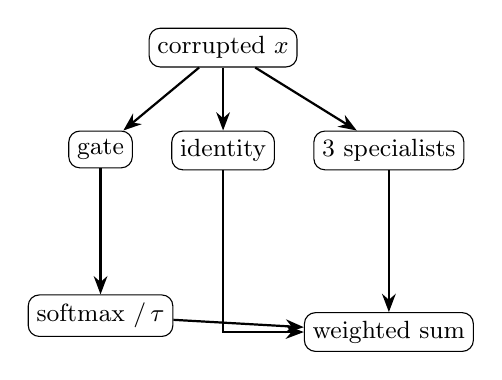
\begin{tikzpicture}[
  box/.style={draw, rounded corners, align=center, font=\small, inner sep=3pt},
  arr/.style={-{Stealth}, thick}
]
\node[box] (x) {corrupted $x$};
\node[box, below left=8mm and 2mm of x] (gate) {gate};
\node[box, below=8mm of x] (id) {identity};
\node[box, below right=8mm and 2mm of x] (exp) {3 specialists};
\node[box, below=16mm of gate] (sm) {softmax $/\,\tau$};
\node[box, below=18mm of exp] (sum) {weighted sum};
\draw[arr] (x) -- (gate);
\draw[arr] (x) -- (id);
\draw[arr] (x) -- (exp);
\draw[arr] (gate) -- (sm);
\draw[arr] (sm) -- (sum);
\draw[arr] (id) |- (sum);
\draw[arr] (exp) -- (sum);
\end{tikzpicture}
\caption{Soft mixture at inference. The gate and specialists start as copies of Task~2.}
\label{fig:mix}
\end{figure}

\section{Losses}
The universal model and each specialist minimize $\alpha \mathrm{L1} + (1-\alpha)(1-\mathrm{SSIM})$ with $\alpha=0.5$. The classifier uses multiclass cross-entropy on class-balanced batches.

The mixture loss is
\begin{equation}
0.8\,\mathrm{L1} + 0.1\,(1-\mathrm{SSIM}) + 0.01\,\mathrm{CE} + 0.01\,B,
\end{equation}
where $B=\sum_{k=1}^{4}(\bar{w}_k-0.25)^2$ and $\bar{w}_k$ is the mean weight of branch $k$ inside the batch. Cross-entropy is computed on the raw gate logits. Temperature only scales the softmax that mixes the experts. The training batches are class-balanced, because otherwise the $0.25$ target does not mean much.

\section{Training procedure}
Optuna was used on Tasks 1, 2, and 3. Those searches were run by the author. The coding agent did not design them and did not launch them.

Task~1 used a fixed setup for the model in the tables, with learning rate $5\times10^{-4}$, batch size 32, and group norm. The plan was 20 epochs. Training was stopped by hand at epoch 15, while the validation score $\mathrm{L1}+(1-\mathrm{SSIM})$ was still going down. The saved epoch has score 0.203. The Optuna file kept with the project is from an earlier bottleneck comparison. That study is the author's, and it is a different network from the one scored below.

For Task~2 the classifier was searched with 10 trials of 5 epochs and no pruner, scoring validation macro-F1. The starting guess that was enqueued won the search. The final classifier then stopped at epoch 12, with validation macro-F1 0.986. The specialist search was meant to be 6 trials of 3 epochs, and it was stopped during trial 5. Trial 0 had the best mean validation score, 0.316. Each specialist was trained after that for 15 epochs at learning rate $5\times10^{-4}$, and all three were still improving when those runs ended.

Task~3 loads those checkpoints and does not start over. The author chose the final hyperparameters after their own Optuna work: temperature 5, batch size 64, loss weights 0.8, 0.1, 0.01, and 0.01, warm-up learning rate $10^{-3}$, and fine-tune learning rate $10^{-4}$. Warm-up freezes the specialists and trains only the gate, for 2 epochs at $10^{-3}$. Fine-tuning then unfreezes the experts and trains everything for 8 epochs at $10^{-4}$. Patience is 4, and a step has to improve the score by at least $10^{-3}$ to count. The longer plan was 20 warm-up epochs and 200 fine-tuning epochs. A longer warm-up had already flattened near validation score 0.150 by epoch 2, and there was not time for 200 fine-tuning epochs. The saved fine-tuning score is 0.133, and it was still falling at epoch 8, so a longer run might do better than what is reported here. The test set was scored once, after this checkpoint had been picked.

Training runs were logged in MLflow. The Optuna studies for the three tasks were run by the author, and the Task~2 databases are the ones saved on disk with trial logs. For the restorers, the validation score is always $\mathrm{L1}+(1-\mathrm{SSIM})$, and lower is better.

\section{Experimental setup}
Every image is $128\times128$ RGB. The reported scores are mean L1, where lower is better, and mean SSIM and PSNR, where higher is better, all against the clean photo. The test set has $3{,}669\times10=36{,}690$ images. ``Do nothing'' means scoring the corrupted input itself. The ONNX files were compared with PyTorch on CPU. The largest absolute gap is $4.6\times10^{-6}$ for Task~1, $6.1\times10^{-6}$ for the specialists, and $3.0\times10^{-6}$ on the mixture image, with $1.2\times10^{-7}$ on its weights.

\section{Results}
\subsection{Task 1}
Fig.~\ref{fig:t1curve} is the training curve up to the early stop, and Fig.~\ref{fig:t1grid} shows validation examples with the clean target, the corrupted input, the reconstruction, and the error. Salt and occlusion beat the input on L1, SSIM, and PSNR. Blur does not. Restored test scores for blur are L1 0.0319, SSIM 0.828, and PSNR 27.2, against an input of 0.0287, 0.829, and 27.8. Low blur is already close to a clean photo, and running it through the bottleneck takes more away than it repairs. Clean images also get worse, with SSIM 0.927, because this model always rewrites the input.

\begin{figure}[t]
\centering
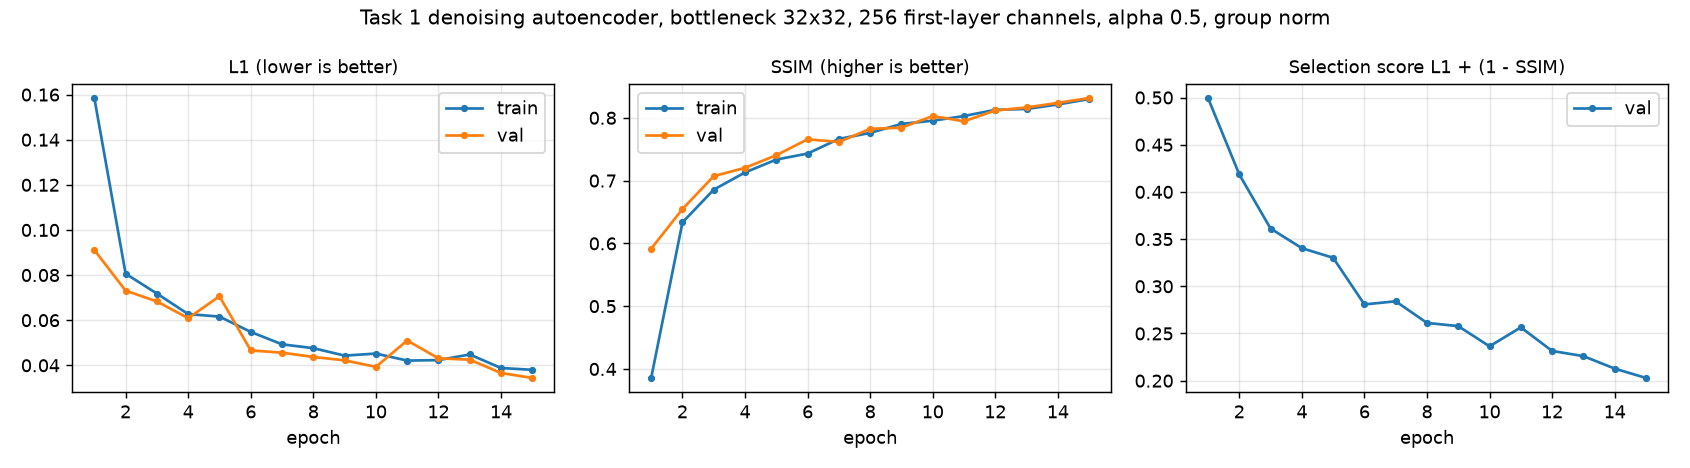
\includegraphics[width=\columnwidth]{figures/loss_curves_dae_b32_a05_gn_20ep.png}
\caption{Task~1 training and validation loss through epoch 15. Validation was still falling when the run was stopped.}
\label{fig:t1curve}
\end{figure}

\begin{figure}[t]
\centering
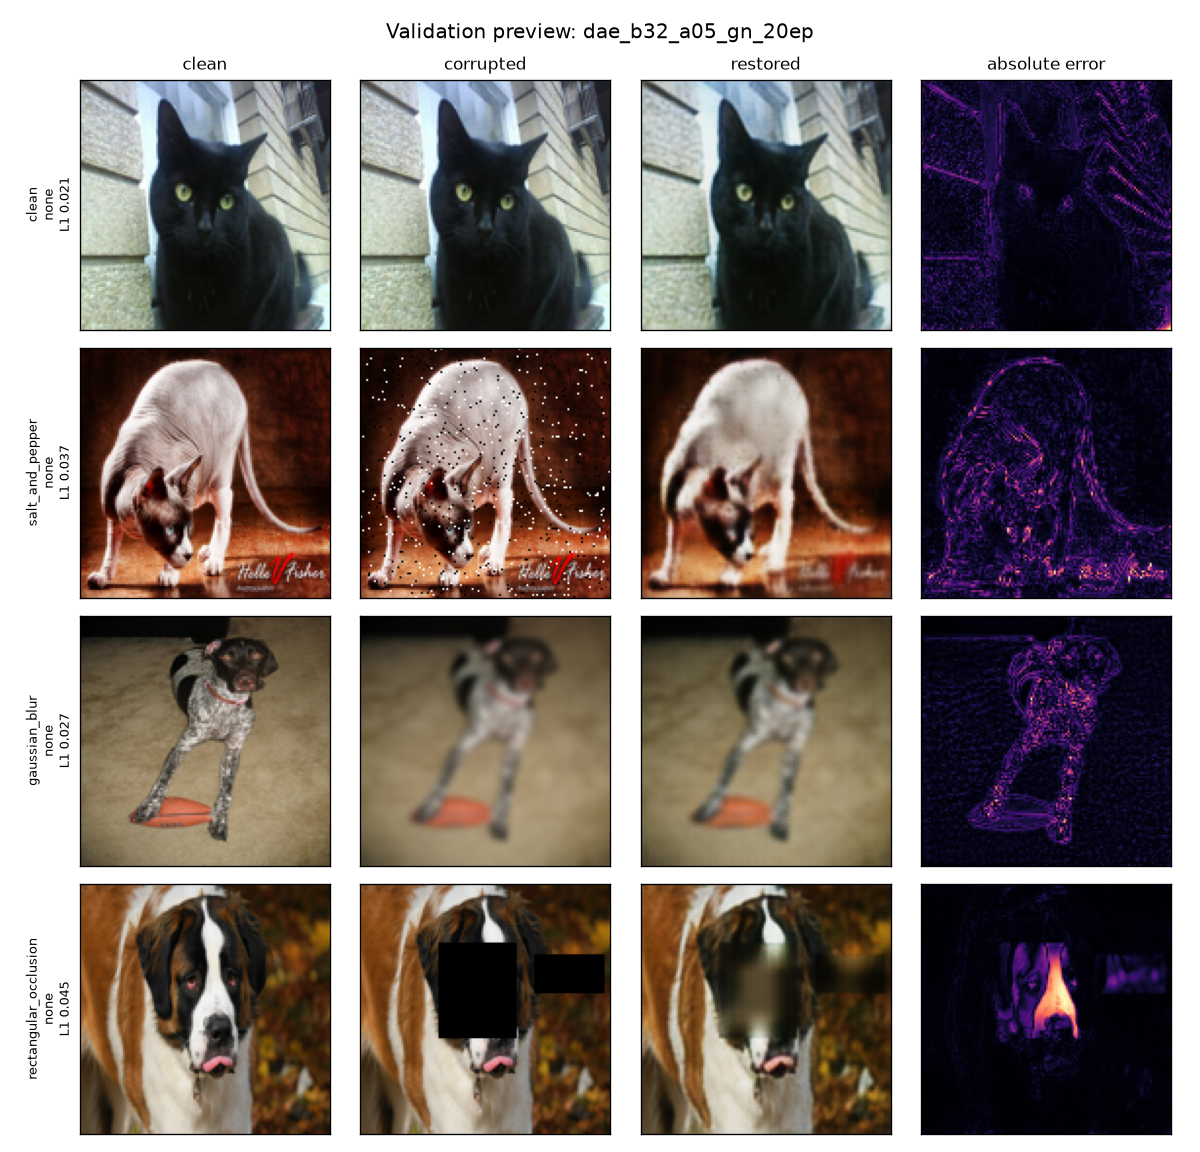
\includegraphics[width=\columnwidth]{figures/val_preview_dae_b32_a05_gn_20ep.png}
\caption{Task~1 validation examples. Each row shows the clean target, the corrupted input, the reconstruction, and the absolute error. The blur rows stay close to the input, since that damage is slight.}
\label{fig:t1grid}
\end{figure}

\subsection{Task 2}
On the test set, accuracy is 0.978 and macro-F1 is 0.965. Salt and blur are close to perfect. The weak cell is low occlusion, where accuracy is 81.5\% and most of the mistakes are called clean, which pulls clean precision down to 0.835. Fig.~\ref{fig:cm} is the normalized confusion matrix.

\begin{figure}[t]
\centering
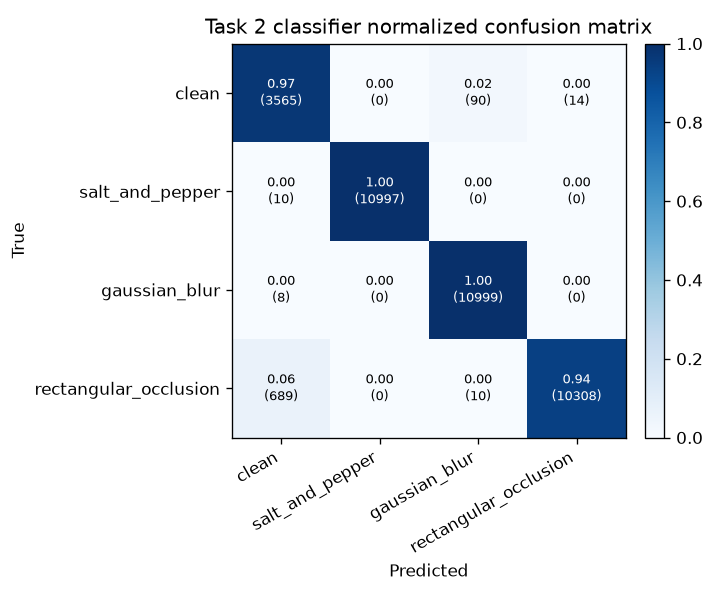
\includegraphics[width=0.9\columnwidth]{figures/confusion_matrix.png}
\caption{Task~2 classifier on the test set. Rows are the true corruption. Most of the off-diagonal counts are low occlusion predicted as clean.}
\label{fig:cm}
\end{figure}

Oracle routing and predicted routing land almost on top of each other, with L1 0.0352 and 0.0351. Wrong routes do not move the average much, because the usual mistake is low occlusion called clean, and the clean bypass then leaves the photo as it is instead of sending it to the wrong specialist. Fig.~\ref{fig:fail} shows some of those predicted-routing cases. Blur still does not beat the input on L1 or PSNR. Clean images stay close to perfect, and that is the main gain over Task~1.

\begin{figure}[t]
\centering
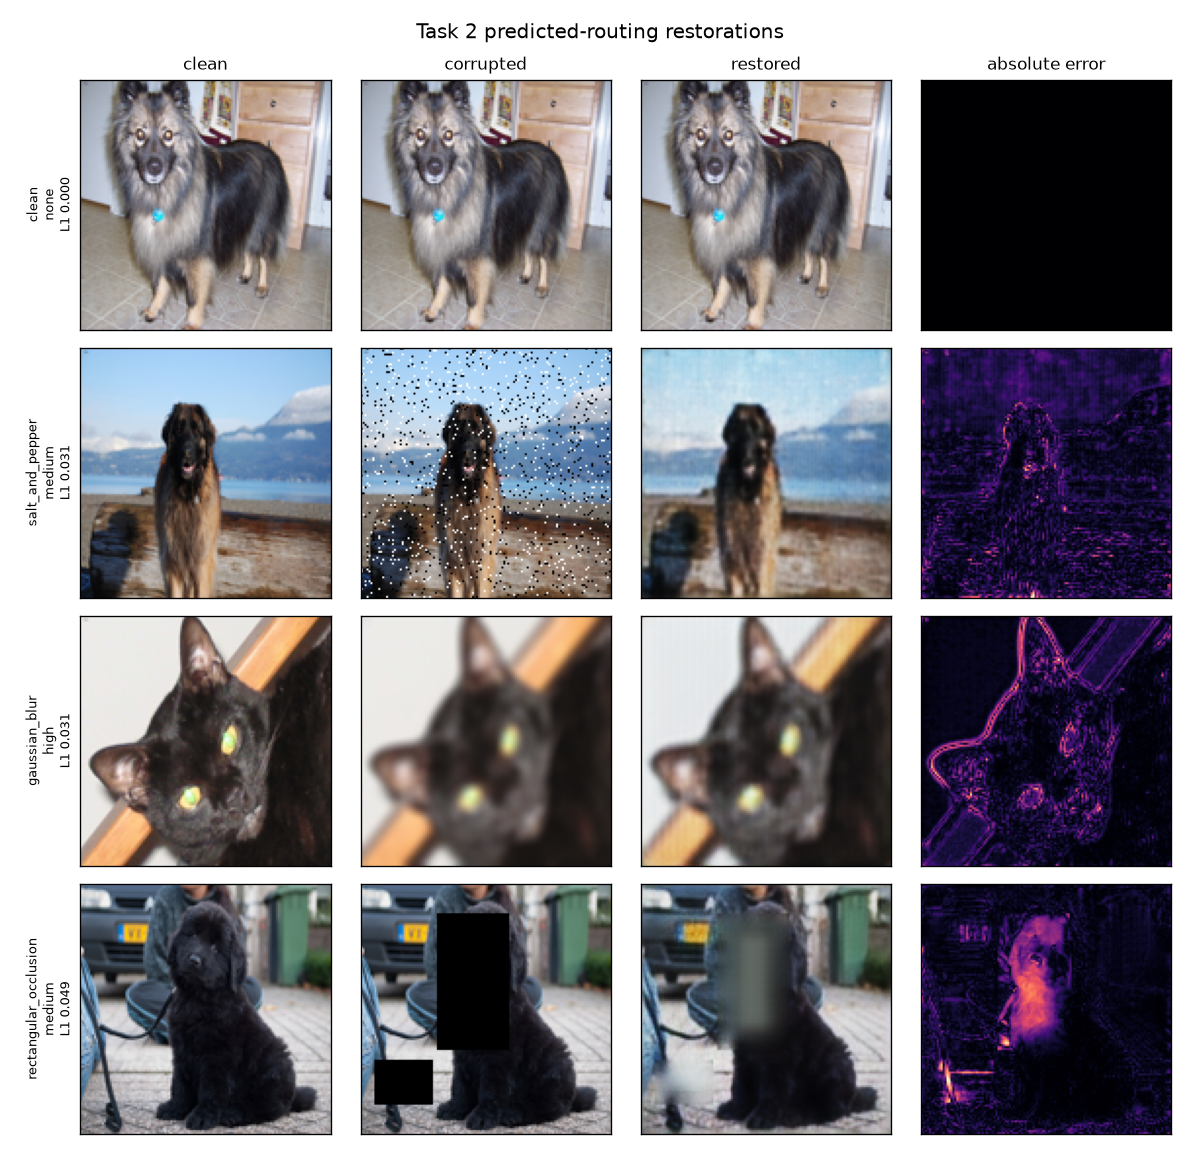
\includegraphics[width=\columnwidth]{figures/predicted_examples.png}
\caption{Task~2 predicted routing. When light occlusion is called clean, the black rectangle stays in the output. That is where the drop in clean precision comes from.}
\label{fig:fail}
\end{figure}

\subsection{Task 3}
Table~\ref{tab:overall} is the average over the whole test set. The mixture is ahead of Task~1 on L1, SSIM, and PSNR. Against hard routing it is ahead on L1 and SSIM, and behind on PSNR.

\begin{table}[t]
\caption{Mean test metrics. L1 lower is better. SSIM and PSNR higher are better.}
\label{tab:overall}
\centering
\begin{tabular}{@{}lccc@{}}
\toprule
System & L1 & SSIM & PSNR \\
\midrule
Do nothing & 0.0506 & 0.695 & 25.3 \\
Task 1 & 0.0381 & 0.806 & 25.3 \\
Task 2, predicted & 0.0351 & 0.843 & 30.5 \\
Task 3 mixture & \textbf{0.0291} & \textbf{0.863} & 28.7 \\
\bottomrule
\end{tabular}
\end{table}

Table~\ref{tab:by} splits the mixture by corruption, with the three severities averaged together. Salt, blur, and occlusion are all better than both earlier restorers. On blur, the three-severity average finally beats the corrupted input, at 0.0279, 0.853, and 28.3 against 0.0287, 0.829, and 27.8. Low blur on its own still loses, with L1 0.0203 against an input L1 of 0.0157. The average only wins because medium blur and high blur improve enough to cover that.

\begin{table}[t]
\caption{Task~3 test means by corruption. Clean has no severity.}
\label{tab:by}
\centering
\begin{tabular}{@{}lccc@{}}
\toprule
Corruption & L1 & SSIM & PSNR \\
\midrule
Clean & 0.0029 & 0.995 & 50.7 \\
Salt and pepper & 0.0268 & 0.871 & 28.4 \\
Gaussian blur & 0.0279 & 0.853 & 28.3 \\
Occlusion & 0.0412 & 0.819 & 22.1 \\
\bottomrule
\end{tabular}
\end{table}

The PSNR gap against Task~2 comes from the clean images. Hard routing copies a clean photo, and that row has PSNR 78.5. The mixture puts mean weight 0.87 on the identity branch and about 0.13 on the blur and occlusion experts, so clean PSNR drops to 50.7. That one row is enough to pull PSNR down across all 36{,}690 images, even though every damaged class is better under the mixture.

Fig.~\ref{fig:heat} shows the mean gate weight for each true corruption and each severity. None of the experts is unused. The overall mean weights are 0.22, 0.29, 0.23, and 0.27. On every true class, the matching branch still has the highest mean weight. Salt and high occlusion sit above 0.99 on the matching expert. Low blur shares the weight, with 0.69 on blur and 0.29 on clean. Low occlusion does the same, with 0.63 on occlusion and 0.34 on clean, which fits the classifier missing light rectangles. Fig.~\ref{fig:dom} shows images where one expert takes most of the weight. A second grid, for cases where the weight is shared, is saved with the project results.

\begin{figure}[t]
\centering
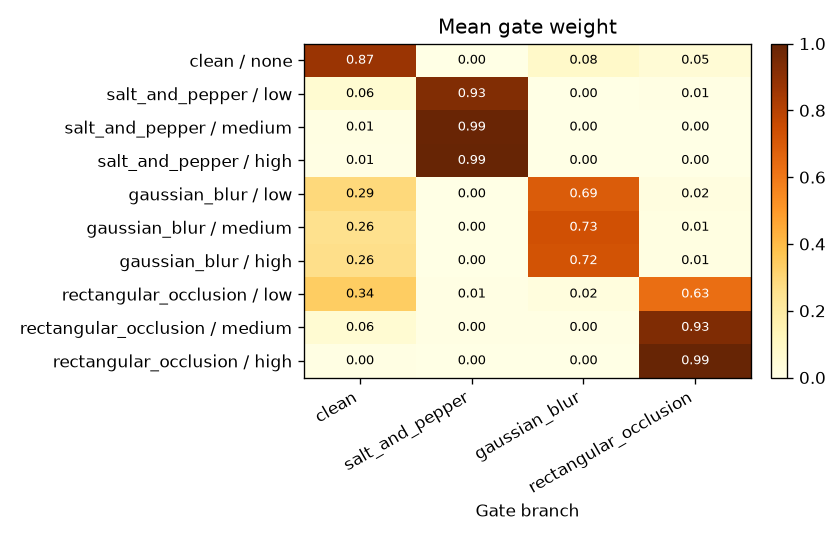
\includegraphics[width=\columnwidth]{figures/weight_heatmap.png}
\caption{Mean Task~3 gate weight on the test set. Rows are the true corruption and severity, and columns are the four branches. The bright cells are the matching expert. Low blur and low occlusion also put weight on clean.}
\label{fig:heat}
\end{figure}

\begin{figure}[t]
\centering
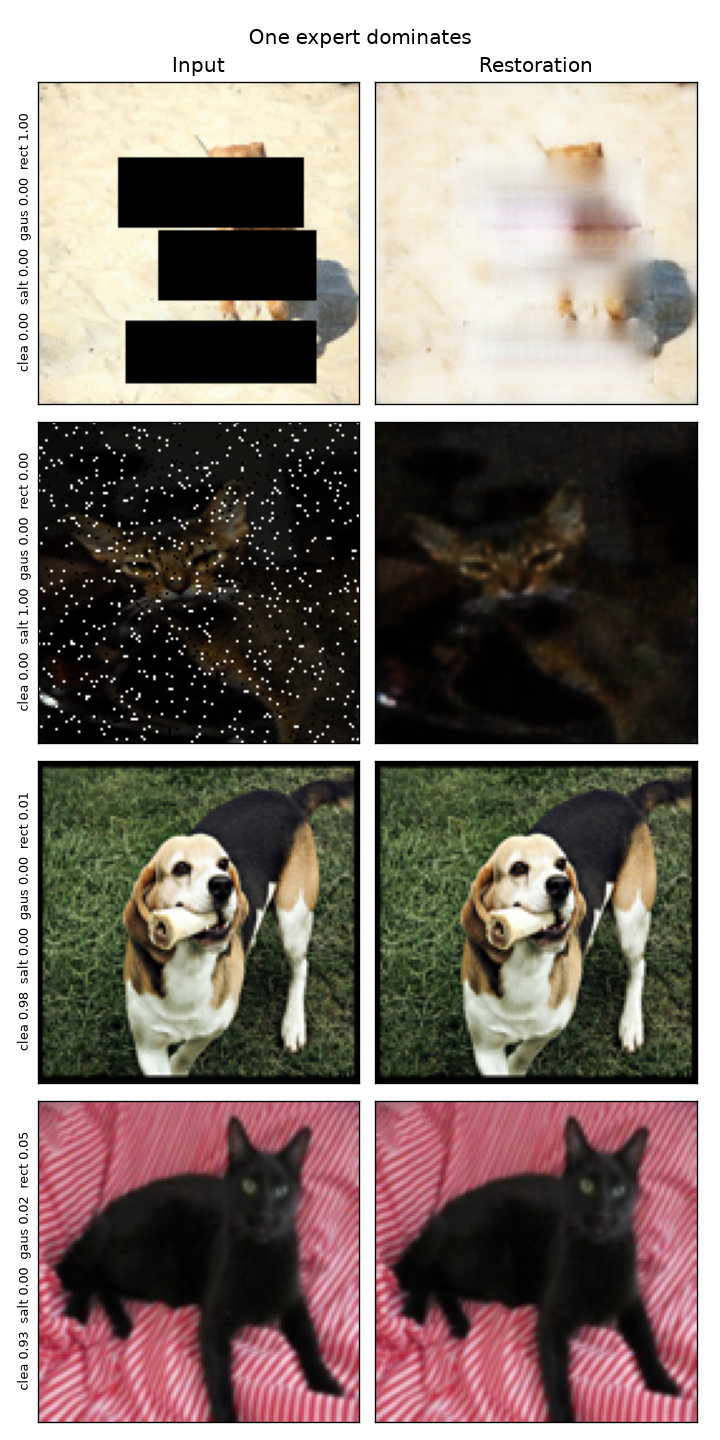
\includegraphics[width=\columnwidth]{figures/dominant_examples.png}
\caption{Cases where one expert holds at least 0.70 of the weight. The text under each pair lists the four weights. Salt and heavy occlusion go to one specialist, which is what the gate is supposed to do when the damage is obvious.}
\label{fig:dom}
\end{figure}

\section{Application}
The browser app is one React and Tailwind page with four workspaces, and it only talks to a FastAPI backend. An upload is checked, resized to $128\times128$ RGB in the same way as training, and then run with ONNX. On the soft mixture screen the user sees the restored image, the four weights, a highlight on any branch at or above 0.25, the inference time, and the corruption settings. One checked example, medium salt and pepper, came back with weights summing to 1.000 and 0.996 on salt. \texttt{docker compose up --build} starts the API and the UI, and the ONNX files are read from \texttt{outputs/}. The Task~4 screen is in the app, but it does not draw a sketch, because no generator was exported.

\section{Limitations}
The Task~1 bottleneck does not compress the image. Low blur is still better if it is left alone. Task~3 fine-tuning stopped at epoch 8 while the validation score was still decreasing, so these numbers are probably short of what this same setup would reach with more epochs. Clean PSNR is worse than hard routing, since the identity branch is mixed with the other experts. The specialist search was short, and it was stopped one trial early. Task~4 and the YouTube demo are not done.

\section{Conclusion}
The specialists help when the damage is the kind they were trained on, and for a clean photo the useful move is to leave it alone. Mixing those outputs with a soft gate improves L1 and SSIM again, and on blur the average over severities finally beats the input. The clean copy is less exact than hard routing, and that shows up in PSNR. A longer fine-tune would be the next thing to measure, and there was not time to run it.

\section*{AI-use appendix}
Cursor was used, with an agent in the editor, to write the Task~3 mixture code, the short training run that used the author's chosen settings, the results screen, and a draft of this paper. Optuna on Tasks 1, 2, and 3 was run by the author, not by the agent. The agent did not pick the search spaces, did not start those studies, and did not choose the winning settings. The loss weights and the temperature for Task~3 came from the author's final configuration. The test numbers in the tables were checked against \texttt{results/task3/summary.json}, \texttt{results/task2/routing\_summary.json}, and the notes for Task~1 and Task~2. The ONNX checks come from the training scripts.

GitHub URL: \url{https://github.com/ibbi1020/GenAI-Assignment-1}.

YouTube URL: not recorded. The demo is not part of this submission.

\begin{thebibliography}{9}
\bibitem{vincent2008}
P.~Vincent, H.~Larochelle, Y.~Bengio, and P.-A.~Manzagol, ``Extracting and composing robust features with denoising autoencoders,'' in \emph{Proc. ICML}, 2008.
\bibitem{wang2004}
Z.~Wang, A.~C.~Bovik, H.~R.~Sheikh, and E.~P.~Simoncelli, ``Image quality assessment: From error visibility to structural similarity,'' \emph{IEEE Trans. Image Process.}, vol.~13, no.~4, pp.~600--612, 2004.
\bibitem{jacobs1991}
R.~A.~Jacobs, M.~I.~Jordan, S.~J.~Nowlan, and G.~E.~Hinton, ``Adaptive mixtures of local experts,'' \emph{Neural Comput.}, vol.~3, no.~1, pp.~79--87, 1991.
\bibitem{shazeer2017}
N.~Shazeer \emph{et al.}, ``Outrageously large neural networks: The sparsely-gated mixture-of-experts layer,'' in \emph{Proc. ICLR}, 2017.
\bibitem{parkhi2012}
O.~M.~Parkhi, A.~Vedaldi, A.~Zisserman, and C.~V.~Jawahar, ``Cats and dogs,'' in \emph{Proc. CVPR}, 2012.
\end{thebibliography}

\end{document}
